\fancyhead[LO, RE]{Appréhender la source}

Dans un premier temps, pour entreprendre l'analyse du texte, il est nécessaire de se familiariser complètement avec le corpus sur la forme et sur le fond, dans l'ensemble et en comptant les pages de titres, pour arriver à de premières conclusions, à explorer ensuite plus, par le biais de plusieurs manipulations. Ainsi, nous commençons par étudier, sur la forme, les différentes éditions de l'ouvrage de Beccaria et collectons divers types d'informations à propos des ouvrages, pour voir les différences entre les éditions, les similarités et autres détails qui pourraient importer pour la poursuite de l'étude des textes, avec nos outils de textométrie\index{Textometrie@Textométrie}. Pour réaliser ce travail, nous avons divisé la tâche en deux parties~: tout d'abord, une lecture et une étude approfondie des textes puis un travail basique de ces textes avec deux/trois outils de textométrie\index{Textometrie@Textométrie}.

\section{Prise de connaissance du corpus~: premières lectures et explorations des sources à disposition}
Après avoir lu l'ouvrage en son entier pour connaître complètement le corpus et pouvoir travailler plus facilement par la suite certains des chapitres en connaissance de cause, je me suis intéressée à lire attentivement tous les \textsc{pdf} et les transcriptions préparées pour le séminaire de février, documents qui représentent ma source de travail pour la majorité de la période du stage, sans l'océrisation\index{OCR!ocerisation@océrisation} de nouveaux chapitres. Cette source se compose donc de plusieurs fichiers en quatre langues (italien, français, anglais, allemand), avec entre cinq et huit documents par langue comprenant les pages de garde de chacune des éditions et l'entièreté du chapitre 30-31-36 dans sa version \textsc{pdf} puis dans la version transcrite. L'objectif était donc de lire chacune des versions pour répertorier les premières différences que je pourrais confirmer par la suite, à l'aide de divers outils.

Cette étude s'est faite principalement avec l'observation des \textsc{pdf} que j'avais à disposition \footnote{Lors de la réalisation de cette étude et la production des tableaux, figures, etc., tous les \textsc{pdf} à disposition, n'avaient pas encore été retrouvés. Il est donc possible qu'il manque certaines éditions, pourtant mentionnées dans d'autres chapitres du mémoire.} et j'ai consigné la plupart des détails relevés dans des tableaux pour avoir une vision globale des similitudes et différences entre versions d'une même langue. Tout d'abord, la première observation consistait à lire la page de garde pour voir si des détails se trouvaient dessus pour discerner des micro changements entre les éditions de même langue, outre la date et le lieu d'édition. De ce fait, nous observons notamment l'origine de l'édition lors d'une traduction et par ce moyen, remarquer par exemple si un ouvrage a été traduit directement depuis la version de Beccaria\index{Beccaria, marquis de} ou si les éditeurs se sont basés sur la version faite par Morellet\index{Morellet, Andre@Morellet, André}.
\begin{figure}[H]
    \centering
    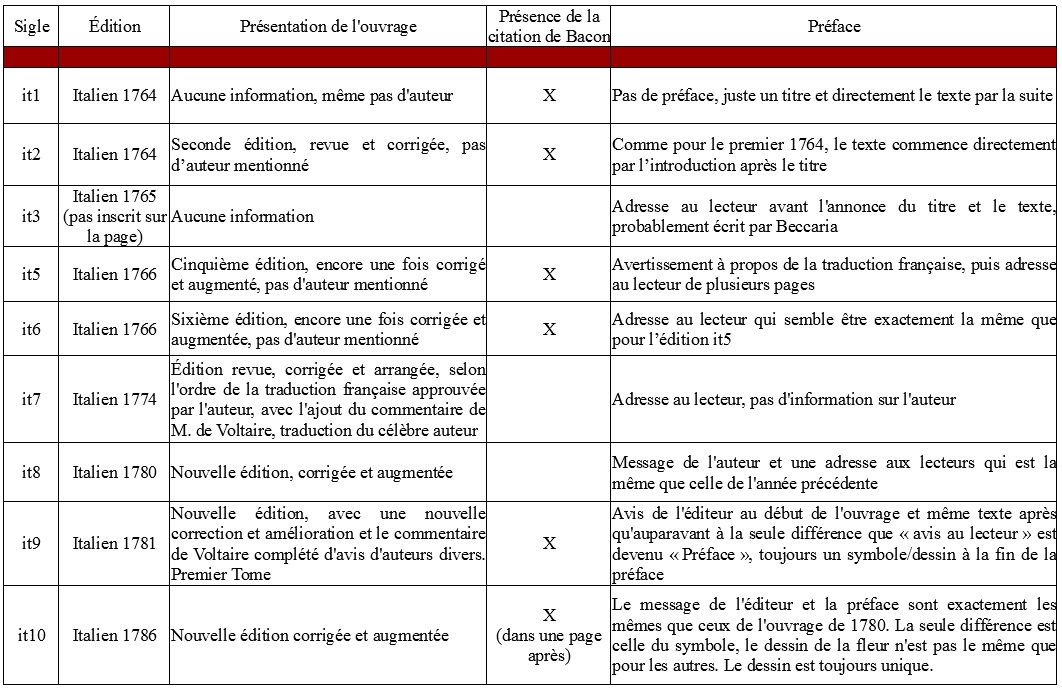
\includegraphics[width=16cm]{Partie3/images/chap1/Editions_it.jpg}
    \caption{Tableau d'observation réalisé pour les pages de garde et préfaces des éditions italiennes}
    \label{fig:editions_it}
\end{figure}
Ensuite, je me suis concentrée sur le contenu même du chapitre donné, pour voir comment le texte a été écrit, pour distinguer les différences d'écriture (si certaines lettres ne sont pas les mêmes qu'aujourd'hui, si les mots sont désuets, etc.), pour constater que certains des éditeurs avaient effectué des changements, que ce soit en insertion de notes de bas de page comme cela peut être le cas pour la majorité des éditions allemandes ou bien même si le texte a été particulièrement modifié dans sa structure comme c'est le cas avec les éditions produites en français en 1766(fr1-1) et 1797(fr1-2).
\begin{figure}[H]
    \centering
    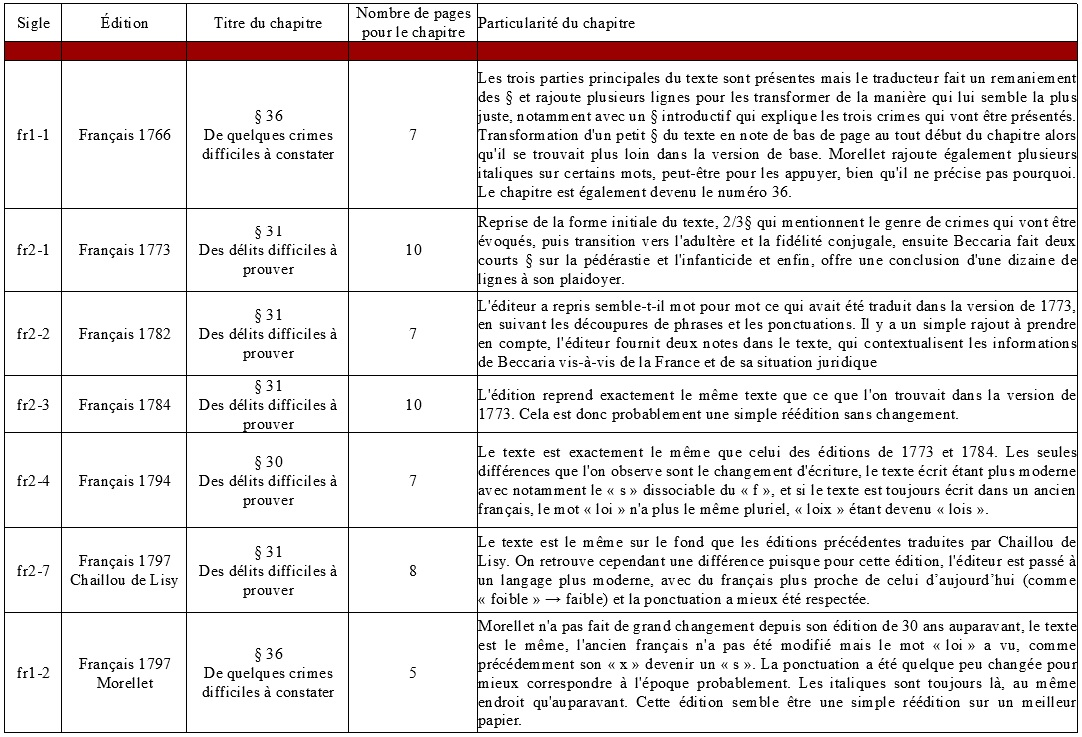
\includegraphics[width=16cm]{Partie3/images/chap1/Chaps_fr.jpg}
    \caption{Tableau d'observation réalisé pour le chapitre 30/31/36 des éditions françaises}
    \label{fig:editions_fr}
\end{figure}
Une fois ces observations faites, nous pouvons tirer de premières conclusions. Il est déjà possible de remarquer que Morellet\index{Morellet, Andre@Morellet, André} a réalisé de grands changements dans le chapitre 30/31, devenu 36 pour lui, et qu'il ne semble plus y avoir de grandes similarités sur la structure du texte et même sur la manière dont les idées sont présentées. Si, dans le fond, ce qui est dit est fondamentalement la même chose, les tournures de phrases ne sont plus les mêmes, l'ordre de présentation des éléments semble avoir changé et il parait donc qu'il n'y a plus le même texte. Ensuite, nous pouvons aussi distinguer les changements apportés par les versions allemandes, qui sont composées en grande majorité de notes de bas de page. Ces notes semblent différer en fonction des éditions, puisque parfois elles sont explicatives pour donner plus de détails à ce qui est présenté et d'autres fois, elles reprennent des morceaux de texte trouvés dans d'autres versions allemandes. Enfin, la dernière observation, essentielle dans la recherche car liée à notre objectif d'établir une généalogie des éditions, est qu'un certain nombre de ces textes sont des rééditions~: la version de 1797 de Morellet\index{Morellet, Andre@Morellet, André} est une réédition de l'ouvrage de 1766 avec quelques modernisations de l'écriture et de termes~; les éditions anglaises d'après 1767 semblent être à chaque fois des rééditions de cette première version~; la version italienne de 1786 est rééditée depuis la version de 1780~; enfin, en allemand, l'édition de 1786 apparaît comme une stricte réédition de la version de 1778. \pagebreak

Ainsi, à travers tout cet examen des textes à disposition, il est déjà possible de cerner une partie des textes et leurs spécificités qui pourront être approfondies postérieurement. Cela permet d'établir une base de connaissances sur les textes qu'il sera possible de développer, d'argumenter ou de modifier avec l'utilisation des outils d'analyse textuelle.

Cette base de connaissances permet néanmoins déjà de répondre à un des objectifs fixés pendant le stage, à savoir la généalogie des éditions et des traductions. En effet, les membres du projet, aidés par le travail réalisé par Philippe Audegean\footcite[p.~33-117]{beccaria_audegean_2009}, avaient déjà regroupé des informations à propos des éditions qui permettaient de se faire une première idée de cette généalogie (informations que nous pouvons retrouver dans les tableaux \ref{table:editions}) et les observations supplémentaires faites pendant cette lecture du texte donnent la possibilité de réaliser cette généalogie, en regroupant toutes les informations à dispositions.
\begin{figure}[H]
    \centering
    \fbox{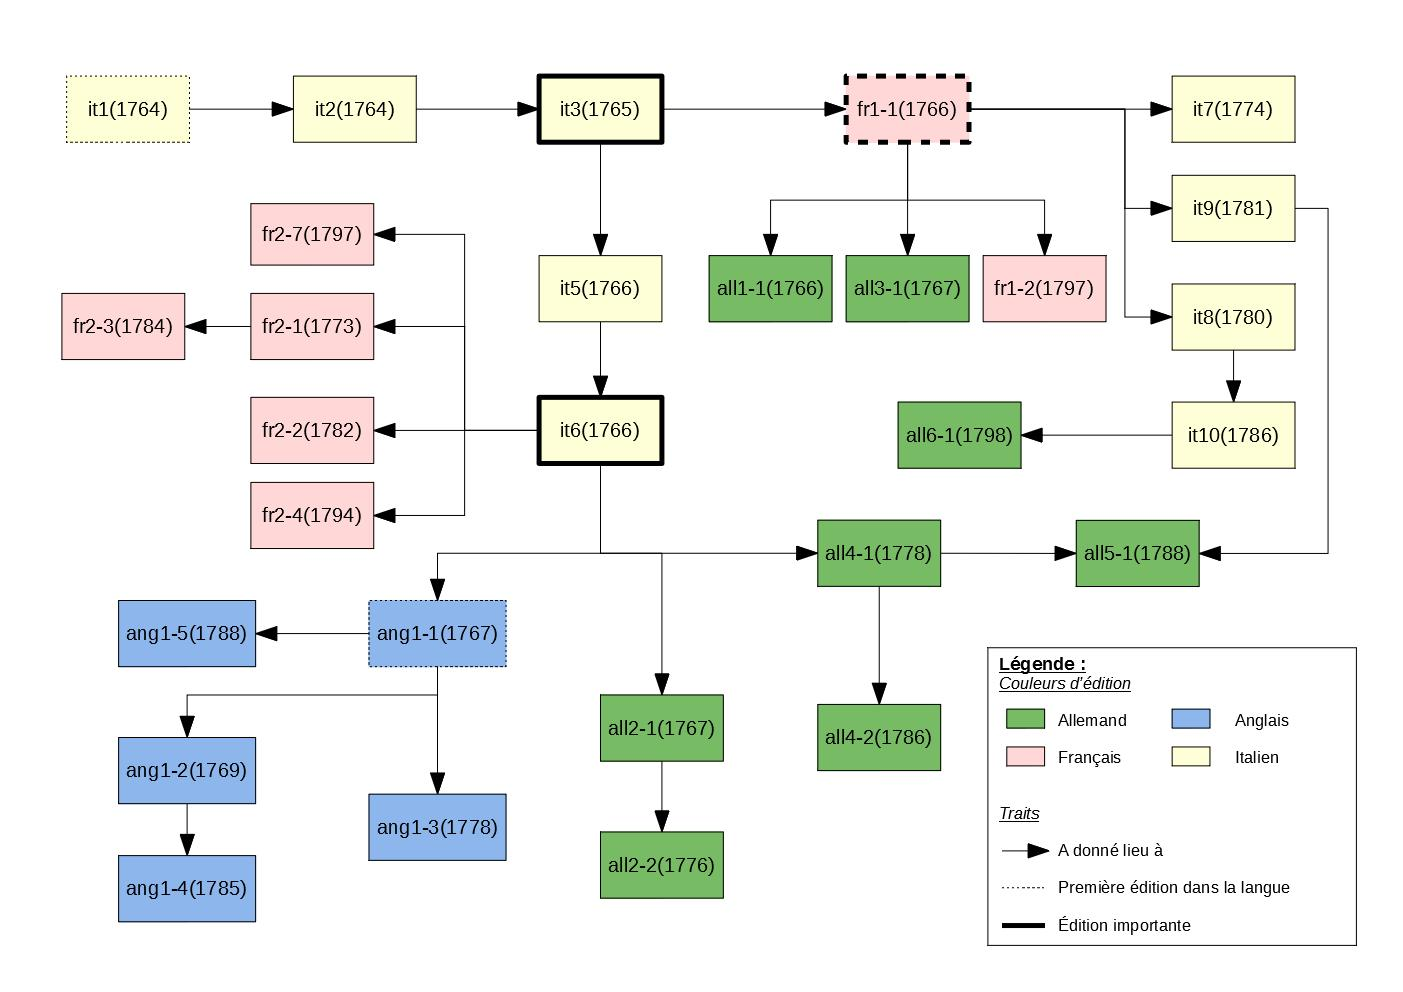
\includegraphics[width=15cm]{Partie3/images/chap1/genealogie.jpg}}
    \caption{Généalogie des éditions et traductions du \emph{Traité}\index{Traite des delits et des peines@Traité des délits et des peines} de Beccaria en italien, français, allemand et anglais}
    \label{fig:genealogie}
\end{figure}
À l'aide d'une lecture des titres de chaque édition du \emph{Traité}\index{Traite des delits et des peines@Traité des délits et des peines} de Beccaria à disposition et en feuilletant les premières pages de l'ouvrage pour observer la préface, les avis de lecteurs et les commentaires insérés, il est possible d'établir cette généalogie des éditions et traductions du texte pour pouvoir déterminer sur quel texte s'est basé chacun des éditeurs pour établir son édition. En l'état, il s'observe que l'abbé Morellet\index{Morellet, Andre@Morellet, André} est parti de la troisième édition de Beccaria\index{Beccaria, marquis de}, publié en 1765, pour effectuer ses modifications, donnant lieu ensuite à une autre publication française, deux allemandes et quatre publications italiennes. Deux de ces publications ont ensuite servies de base pour produire deux nouvelles éditions allemandes. Le texte a été édité cinq fois en italien avant d'arriver à la sixième édition, qui est le texte de départ pour les éditions anglaises, pour la majorité des textes français et pour deux éditions allemandes. Cette généalogie permet également de distinguer un certain nombre de rééditions d'une même langue, que cela soit le cas pour l'italien, le français, l'anglais ou l'allemand. Enfin, il y a un cas assez unique pour l'édition de  1788, qui se base sur l'édition italienne de 1781 pour son texte mais également sur l'édition allemande publiée en 1778, pour le cas de ses notes de bas de page.

\section{Examens préliminaires des textes de Beccaria~: découvrir les outils d'analyses textuelles}
Une fois les premières lectures effectuées, nous approfondissons notre recherche de base en utilisant quelques outils de textométrie\index{Textometrie@Textométrie} pour essayer de faire ressortir les caractéristiques observées précédemment, pour voir si nos premières conclusions se confirment, si une analyse sur le fond fait apparaître une vision contraire à celle que nous avons eue ou s'il n'y a que des différences légères. Pour réaliser cet examen, nous avons choisi trois outils~: un logiciel à télécharger, \textsc{txm}{\footcite{txm_plateforme}} et deux logiciels présents sur le web, \textsc{juxta commons}{\footnote{\url{http://juxtacommons.org/}}} et \textsc{medite}{\footnote{\url{http://obvil.lip6.fr/medite/}}}.

\subsection{Étudier les dimensions du corpus~: introduction à TXM}
\begin{figure}[t]
    \centering
    \caption{Production \textsc{txm} présentant les dimensions des corpus pour chaque langue par nombre de mots en fonction de chaque édition (haut gauche~: allemand, droit~: anglais, bas gauche~: français, droit~: italien)}
    \fbox{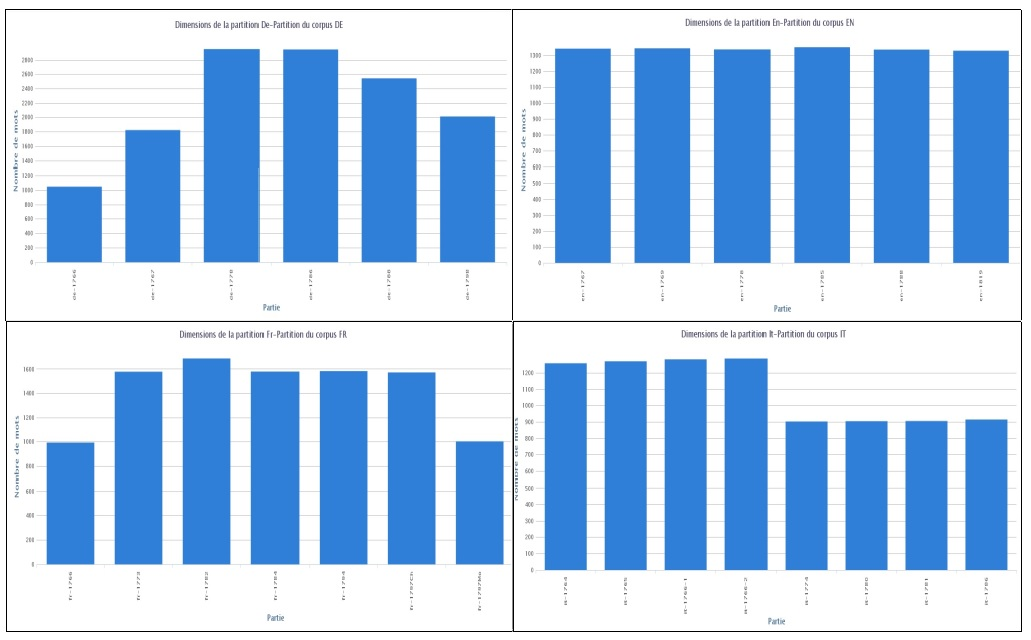
\includegraphics[width=14cm]{Partie3/images/chap1/Dimensions.jpg}}
    \label{fig:dimensions}
\end{figure}
Tout d'abord, nous pouvons vérifier certaines des conclusions à l'aide de \textsc{txm}, qui sera majoritairement utilisé pendant le stage. \textsc{txm} est un outil de textométrie\index{Textometrie@Textométrie} doté d'un certain nombre d'options permettant de faire apparaître divers types d'informations à propos d'un corpus. Parmi ces options, il y a \textbf{\textit{Propriétés}} qui s'applique au corpus ou à une version partitionnée \footnote{Apparition du corpus selon une unité structurelle différente (phrases, texte, etc.) et avec une propriété particulière (par langue, année, numéro de phrase, etc.)} et qui prend en compte le nombre de mots pour chacun des fichiers présents dans le corpus importé. À partir de cela, cet outil fait apparaître, sous forme d'un diagramme en barre, les dimensions du corpus (voir figure \ref{fig:dimensions}). Cette étape est très intéressante puisqu'elle permet de voir la diversité entre les langues et la différence ou non différence en fonction des éditions. Nous observons pour chacune des langues un trait caractéristique, qui va parfois dans le sens de ce qui a déjà été rapporté lors de la lecture du corpus, qui agrémente, d'autres fois, une précédente observation ou enfin, certaines qui nous font contempler des caractéristiques non observées auparavant. Ainsi, concurremment de ce qui avait été vu lors de la lecture du corpus, les éditions anglaises semblent effectivement être des rééditions strictes de la toute première parution, sans changement quel qu'il soit dans le cas du chapitre 31 au moins. Le corpus est constitué d'à peu près le même nombre de mots pour chacune des éditions, à quelques mots près, probablement dû à des erreurs d'\acrshort{ocr}\index{OCR} ou à des changements mineurs. Les autres corpus présentent des différences beaucoup plus flagrantes. Pour le cas de l'italien, il y a une démarcation claire entre les quatre premières éditions et les quatre dernières~: cela est dû à une différence de versions puisque les éditions de 1764, 1765 et les deux de 1766 sont ou reprennent le texte écrit par Beccaria\index{Beccaria, marquis de}, alors qu'à partir de 1774 et après en 1780, 1781 et 1786, la traduction italienne se fait depuis l'édition française créée par Morellet\index{Morellet, Andre@Morellet, André}, avec ses différentes modifications. Par cela s'observe donc le fait que la version de Morellet\index{Morellet, Andre@Morellet, André} supprime un certain nombre de mots dans le chapitre 30 de Beccaria\index{Beccaria, marquis de}, amenant à une traduction plus courte et bien différente, comme cela avait été observé avec la lecture du corpus italien et même français. Vis-à-vis des éditions françaises, nous distinguons également bien la démarcation entre la version de Morellet\index{Morellet, Andre@Morellet, André} et la version de Chaillou de Lisy\index{Chaillou de Lisy, Etienne}, qui traduit en suivant la structure de Beccaria\index{Beccaria, marquis de}. La différence dans le nombre de mots se discerne amplement et expose la divergence entre les deux. L'autre édition qui se détache un peu des autres est celle de 1782, qui semble dépasser d'une centaine de mots le reste des manuscrits non édités par Morellet\index{Morellet, Andre@Morellet, André}, ce qui est minime mais montre un écart. Cela est dû, d'après une recherche subséquente, à des notes de bas de pages intégrées dans cette version. Enfin, la dernière dimension de corpus est le cas de l'allemand qui présente le plus de dissimilitudes entre ses différentes versions. Ces variations semblent venir d'ajouts de notes de bas de pages, qui diffèrent en fonction de chaque version et de changements d'origine de la traduction (parfois Beccaria\index{Beccaria, marquis de}, parfois Morellet\index{Morellet, Andre@Morellet, André}). La seule observation qui confirme nos suppositions précédentes est le fait que la version de 1786 semble effectivement être une réédition de 1778, puisque l'outil atteste du même nombre de mots entre les deux.

Par cet outil, nous pouvons donc déjà contempler une certaine quantité de caractéristiques à propos du corpus, ce qui nous aide à mieux approfondir nos connaissances sur sa composition et sa structure, élément utile lorsqu'il sera étudié plus intérieurement.

\subsection{Comparer les textes entre eux~: manipulations avec Juxta Commons}
Nous pouvons ensuite passer à une étude plus portée sur le fond du texte et notamment sur les changements effectués dans les éditions au fur et à mesure des parutions. \textsc{juxta commons} est un outil parfait pour cela puisqu'une fois que le corpus lui est soumis, il le collationne et fait ensuite apparaître les textes sous différentes formes, telle que la \og~Heat Map~\fg{}, qui prend un texte de base et présente toutes les différences par rapport aux autres textes du corpus. La \og~Side-by-side view~\fg{}, autre option, sélectionne deux textes du corpus soumis et expose les différences entre les deux. Il y a aussi la \og~parallel-segmentation~\fg{} qui produit une édition critique en \textsc{xml} contenant tous les textes et des identifiants et témoins pour observer, selon un témoin de base, les endroits du texte où il y a une différence et comment celle-ci apparaît pour chacune des versions. Ces trois options sont les plus utiles pour faire ressortir les informations voulues. En majorité, l'utilisation de \textsc{juxta commons} a permis de faire ressortir ce qui avaient déjà été observés lors des premières explorations. La \og~parallel-segmentation~\fg{} est un outil parfaitement adapté pour les éditions anglaises puisque, comme nous le voyons, il n'y a que très peu de balises <rdg> (balises servant à faire ressortir les différences)~; généralement, ces différences sont dues à des erreurs d'\acrshort{ocr}\index{OCR} qui ont rendu un des mots incorrects dans une des versions. Cet outil démontre donc que l'anglais n'a que très peu de changements entre ses éditions. Le français et l'italien font très vite apparaître de grandes différences entre les versions mais cela est minimisé dès que sont créés des sous-corpus en fonction de l'origine des traductions~: d'un côté, les éditions avec la structure de Beccaria\index{Beccaria, marquis de} et de l'autre, les éditions avec celle de Morellet\index{Morellet, Andre@Morellet, André}. Une fois cela exécuté, nous ne remarquons que très peu de différences, à part des changements d'écriture avec des apparitions d'accents sur les mots pour l'italien et des modernisations de mots pour les deux langues. Enfin, les éditions allemandes sont peu adaptées à la \og~parallel-segmentation~\fg{} car les différences sont beaucoup trop importantes, de même pour la \og~side-by-side view~\fg{} qui montrera d'énormes changements entre les deux versions. Cela ne nous apporte qu'une confirmation de ce que nous avions conclu, à savoir que les éditions sont fondamentalement différentes, sauf, encore une fois, 1778 et 1786. Toutes ces considérations peuvent s'observer avec une des vues de la \og~Heat Map~\fg{} prenant l'édition de 1778 comme édition de base, qui montre que les différences entre les autres textes sont immenses et qu'il y en a même dans le cas de la réédition de 1786.
\begin{figure}[H]
    \centering
    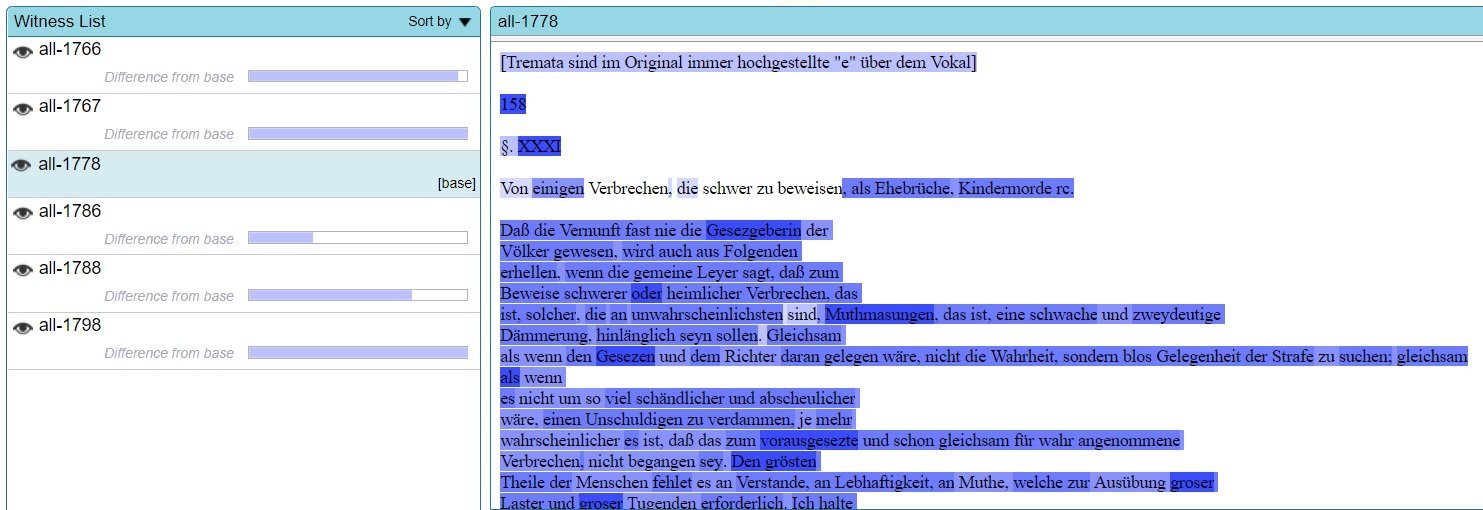
\includegraphics[width=16cm]{Partie3/images/chap1/Heat_Map.jpg}
    \caption{Démonstration des différences entre les éditions allemandes avec 1778 comme édition de base par la \og~Heat Map~\fg{} produite par \textsc{juxta commons}}
    \label{fig:heat_map}
\end{figure}
Ainsi, \textsc{juxta commons} est un outil pratique pour nos premières recherches puisqu'il confirme ce qui avait été supposé sur notre texte, les différences en fonction des langues, les similarités pour certaines des éditions et il est possible de discerner un semblant de schéma. Les éditions anglaises et allemandes sont à des opposés~: les premières ont un corpus quasi-identique alors que les secondes ont des caractéristiques particulières pour chacune des éditions. Au centre de ce schéma, se trouvent les corpus italiens et français qui ne diffèrent globalement qu'en fonction de l'origine des traductions.

\subsection{Confirmer ou non les observations précédentes~: l'analyse par MEDITE}
Pour finir notre travail préliminaire, un troisième outil d'analyse de texte est utilisé~: \textsc{medite}, un logiciel d'alignement\index{Alignement} de textes développé par le laboratoire d'excellence de l'\acrfull{obvil}. Il permet d'observer les suppressions, insertions, remplacements et déplacements entre deux textes et est donc une bonne base pour notre travail qui sera également un alignement\index{Alignement} de textes, mais il ne permet pas de réaliser un alignement multilingue\index{Alignement!alignement multilingue}, notre objectif. \textsc{medite} est assez similaire à la \og~side-by-side view~\fg{} de \textsc{juxta commons} mais le logiciel donne la possibilité de choisir des options d'affichage tel qu'une sensibilité à la casse ou une option pour qu'il ne fasse apparaître que les blocs en commun. Une fois les textes chargés, nous pouvons alors observer les variations avec des précisions indiquées sur le côté des textes, comme le montre la figure \ref{fig:medite}.
\begin{figure}[H]
    \centering
    \fbox{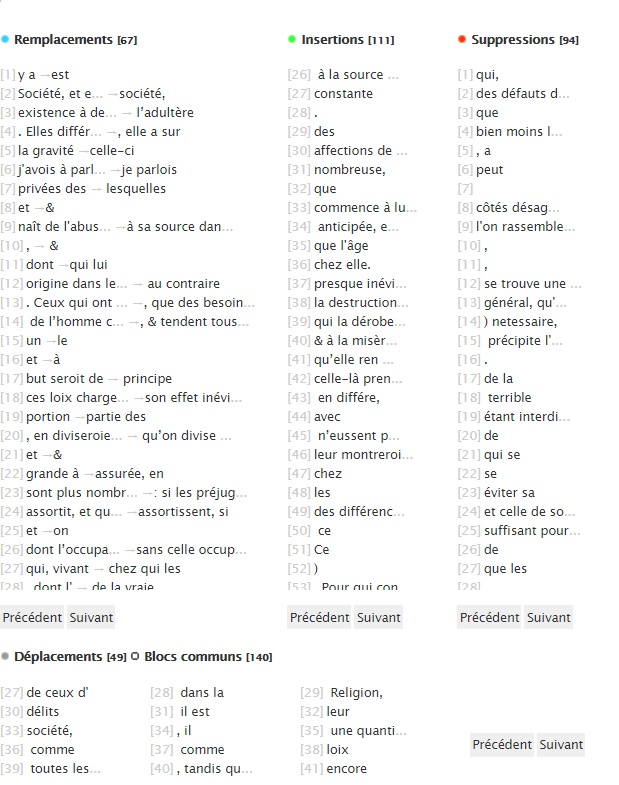
\includegraphics[width=15cm]{Partie3/images/chap1/MEDITE_alignement.jpg}}
    \caption{Alignement\index{Alignement} de textes~: présentation des remplacements, insertions, suppressions, déplacements et blocs communs entre le chapitre 30/31/36 des éditions françaises de 1766 et 1773}
    \label{fig:medite}
\end{figure}
L'outil est assez complet puisque nous pouvons observer les numéros de lignes où apparaissent ces changements, les différences quand il s'agit de remplacements et même le nombre de ces changements pour chaque catégorie.

Ce logiciel est bien adapté puisqu'il permet de vérifier les conclusions faites lors des examens précédents du texte. Nous pouvons ainsi choisir deux textes qui présentent ou non des altérités pour chacune des langues et alors constater si nos suppositions s'avèrent vraies. L'analyse suivante nous montre que cela n'est pas exactement le cas et que les textes ne sont pas toujours si différents que présumés.
\begin{figure}[H]
    \centering
    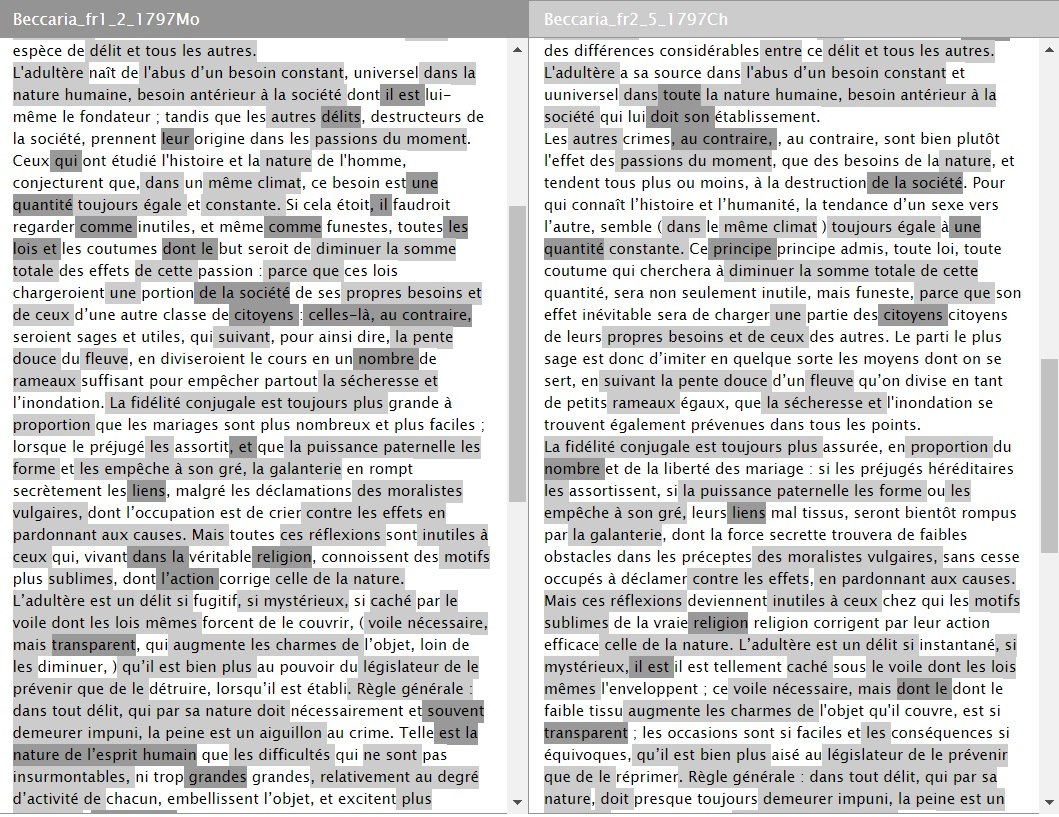
\includegraphics[width=15cm]{Partie3/images/chap1/MEDITE_fr.jpg}
    \caption{Alignement\index{Alignement} de textes entre l'édition française de 1797 de Morellet\index{Morellet, Andre@Morellet, André} et celle de 1797 de Chaillou\index{Chaillou de Lisy, Etienne}}
    \label{fig:medite_fr}
\end{figure}
En décidant de ne faire apparaître que les blocs communs entre une édition reprenant la structure de Morellet\index{Morellet, Andre@Morellet, André} et une reprenant celle de Beccaria\index{Beccaria, marquis de}, nous pouvons voir que les changements effectués par Morellet\index{Morellet, Andre@Morellet, André} ne sont pas si conséquents. Il semble avoir opérer un certain nombre de déplacements de paragraphes ou de groupes de mots, pour présenter le texte selon ce qu'il pensait être le mieux mais ces groupes de mots restent cependant les mêmes que ceux traduits depuis l'édition de Beccaria\index{Beccaria, marquis de}. Nous pouvons, de plus, confirmer ces observations avec le tableau \ref{table:alignement_medite_fr}, où nous avons fait une comparaison cette fois entre la première édition de Morellet\index{Morellet, Andre@Morellet, André} en 1766 et la première reprenant la structure de Beccaria\index{Beccaria, marquis de}. Nous pouvons voir qu'il y a eu un certain nombre de changements dont notamment des suppressions et quelques déplacements, mais le tableau montre tout de même une quantité de blocs communs (130). Le résultat du logiciel ne démonte pas complètement la théorie avancée, puisque les deux types d'éditions présentent effectivement un certain nombre de variations, même dans le cas des paragraphes où les idées sont les mêmes. La différence majeure est la suppression de deux paragraphes d'explications qu'avait inséré Beccaria\index{Beccaria, marquis de} au début du chapitre et qui ont été supprimés par Morellet\index{Morellet, Andre@Morellet, André}, ce qui s'observe ici par le biais de la barre de défilement qui est plus courte pour la version de Morellet\index{Morellet, Andre@Morellet, André}. Cela démontre un texte plus court que la version 1797 de Chaillou\index{Chaillou de Lisy, Etienne}. André Morellet\index{Morellet, Andre@Morellet, André}, dans sa traduction, semble avoir ensuite reformulé les idées, pour être plus direct dans son approche et exposer plus rapidement ses idées. Le tableau \ref{table:alignement_medite_fr} présente également, avec sa troisième et quatrième colonne, le fait que Morellet\index{Morellet, Andre@Morellet, André} a bien effectué une réédition en 1797, mais qu'il n'a pas changé beaucoup d'éléments, comme le montre les chiffres du tableau, notamment lorsque les séparateurs ne sont pas pris en compte. 

\begin{table}[H]
\centering
\begin{tabular}{|c|c|c|c|c|}
\hline
 & 1766 vs 1773 & 1766 vs 1773 & 1766 vs 1797Mo & 1766 vs 1797Mo \\
 & (avec s.) & (sans s.) & (avec s.) & (sans s.) \\ \hline
Remplacements & 67 & 62 & 53 & 52 \\ \hline
Insertions & 111 & 95 & 15 & 1 \\ \hline
Suppressions & 94 & 78 & 7 & 0 \\ \hline
Déplacements & 49 & 40 & 0 & 0 \\ \hline
Blocs Communs & 140 & 130 & 72 & 54 \\ \hline
\end{tabular}
\caption{Données de l'alignement entre les éditions françaises de 1766 et 1773 et 1766 et 1797 (Morellet), avec le comptage des séparateurs (!,;.?...) et sans}
\label{table:alignement_medite_fr}
\end{table}

C'est avec l'étude des versions italiennes que l'impact de \textsc{medite} est beaucoup plus important et significatif pour nos suppositions antérieures, comme le tableau \ref{table:alignement_medite_it} et la figure \ref{fig:medite_it} nous permettent de l'observer.
\begin{table}[H]
\centering
\begin{tabular}{|c|c|c|}
\hline
 & 1766 vs 1774 (avec s.) & 1766 vs 1774 (sans s.) \\ \hline
Remplacements & 53 & 36 \\ \hline
Insertions & 46 & 3 \\ \hline
Suppressions & 68 & 4 \\ \hline
Déplacements & 0 & 0 \\ \hline
Blocs Communs & 164 & 41 \\ \hline
\end{tabular}
\caption{Données de l'alignement entre les éditions italiennes de 1766 et 1774, avec le comptage des séparateurs (!,;.?...) et sans}
\label{table:alignement_medite_it}
\end{table}

\begin{figure}[H]
    \centering
    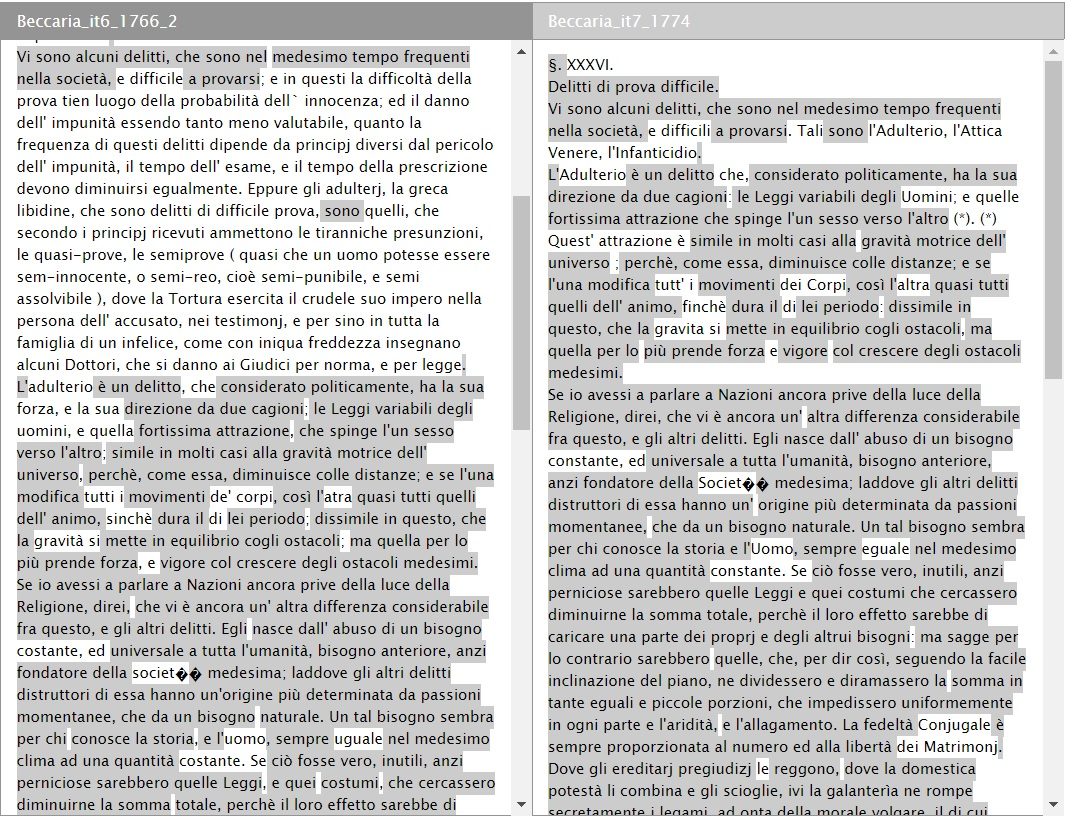
\includegraphics[width=15cm]{Partie3/images/chap1/MEDITE_it.jpg}
    \caption{Alignement\index{Alignement} de textes entre les éditions italiennes de 1766 et 1774}
    \label{fig:medite_it}
\end{figure}

L'édition de 1766 suit ce qui avait été écrit par Beccaria\index{Beccaria, marquis de} alors qu'à partir de l'édition de 1774, le \emph{Traité}\index{Traite des delits et des peines@Traité des délits et des peines} suit les changements effectués par Morellet\index{Morellet, Andre@Morellet, André}, avec une traduction italienne de la traduction française. Par le biais de ces colorations de blocs en commun, il est possible de voir que les deux versions italiennes ne sont pas aussi éloignées que nous le présumions. Il y a toujours le cas de ces deux premiers paragraphes de présentation que Morellet\index{Morellet, Andre@Morellet, André} a réduit, ce qui se matérialise probablement par la suppression de quatre blocs dans le tableau \ref{table:alignement_medite_it} mais outre cela, il y a de très grandes similitudes entre les deux textes, voire même une égalité puisque les remplacements qui ressortent semblent majoritairement dues à des erreurs d'\acrshort{ocr}\index{OCR}, à des majuscules ou à des espaces qui ne sont pas à la même place. Les insertions sont assez minimes, hors prise en compte des séparateurs et les déplacements sont inexistants. Ainsi, si les différences en français se justifiaient par des reformulations de la part du traducteur, le traducteur italien semble avoir repris la structure de Morellet\index{Morellet, Andre@Morellet, André} sans changer l'intérieur du texte lorsque cela n'avait pas été le cas en français. L'éditeur italien de 1774 arrive ainsi à un résultat qui diffère de la version originale mais pas autant que cela avait pu être supposé lors des analyses de lecture et de \textsc{juxta commons}.

Ainsi, \textsc{medite} est un très bon outil pour terminer l'analyse préliminaire puisqu'il donne la possibilité de remettre en question certaines des conclusions établies lors des précédentes observations avec les corpus italien et français notamment, puisqu'il démontre que les différences ne sont pas aussi grandes que nous le pensions. Cela aidera pour la suite du travail puisque nous pourrons aborder l'alignement multilingue\index{Alignement!alignement multilingue} avec une autre perception et avec l'idée que cela est possible dans certains cas. Les disparités ne sont pas aussi évidentes et les comparaisons pourront donc être effectives. Les deux autres langues ont également été passées à travers \textsc{medite}~; l'analyse de l'allemand reprend seulement ce qui a déjà été observé avec \textsc{juxta commons} notamment et cela prendrait un temps inutile d'essayer de voir les différences entre toutes les versions pour arriver à la conclusion qu'ils ne ressemblent asbolument pas~; l'analyse de l'anglais confirme ce qui a déjà été supposé, les différences sont infimes entre les versions (cas de majuscules, d'espaces, de virgules, etc.).

\paragraph{}Ces différents examens et analyses effectués sur le texte nous ont donc permis d'approfondir nos connaissances sur le corpus, sur sa composition et son contenu~; malgré l'aspect assez basique et préliminaire de cette étude, nous pouvons déjà nous faire une idée des obstacles qui se présenteront dans la mise en place de l'alignement de texte, tel que les multiples structures de texte, qui pourraient être embarrassantes. L'intérêt surtout de cette étude est de montrer la diversité des outils à disposition pour faire des analyses et leur nécessité également, puisque les résultats ne sont pas toujours les mêmes en fonction du logiciel utilisé. Ces outils se complètent et permettent, même à un niveau de travail peu approfondi comme celui-ci, de faire apparaître des éléments nécessaires pour connaître correctement son corpus et continuer le travail à partir de là.

Les observations faites sont essentielles pour notre étude de la source et permettent ainsi de mieux appréhender les tâches à venir, qui se concentreront sur un aspect plus précis du corpus documentaire, à savoir les termes juridiques qui ponctuent le texte et qui seront le fil conducteur de notre alignement\index{Alignement}. 